% DO NOT COMPILE THIS FILE DIRECTLY!
% This is included by the other .tex files.

\begin{frame}[t,plain]
  \titlepage
\end{frame}

%---------------------------------------------------------------------
\section{Problem Overview \& Motivation}

%\begin{frame}[t]{MagLIF}
%  8 minutes
%  \begin{itemize}
%    \item What is MagLIF?
%    \item How does it work?
%    \item What makes it interesting to us?
%    \item What can you draw from Literature?
%    \item Where is our Investigation?
%    \item What are still issues that they have with MagLIF? (See Tech-X talk)
%    \item How does what we do "Kinetic Closures" help with the fluid model
%  \end{itemize}
%
%\end{frame}
\begin{frame}[t, label=current]{Direct Drive - 1}
 \begin{figure}[!htbp]
   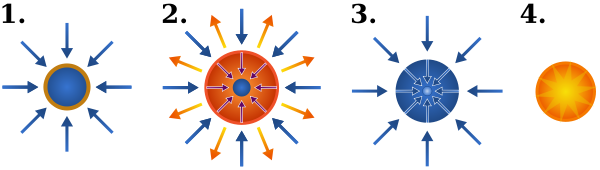
\includegraphics[width=0.8\linewidth]{fig/600pxICF.png}
   \centering
 \end{figure}
 \footnote{Inertial Confinement Fusion Wiki}
\end{frame}


\begin{frame}[t, label=current]{Direct Drive - 2}
  \vspace{-0.5cm}
  \begin{figure}[!htbp]
   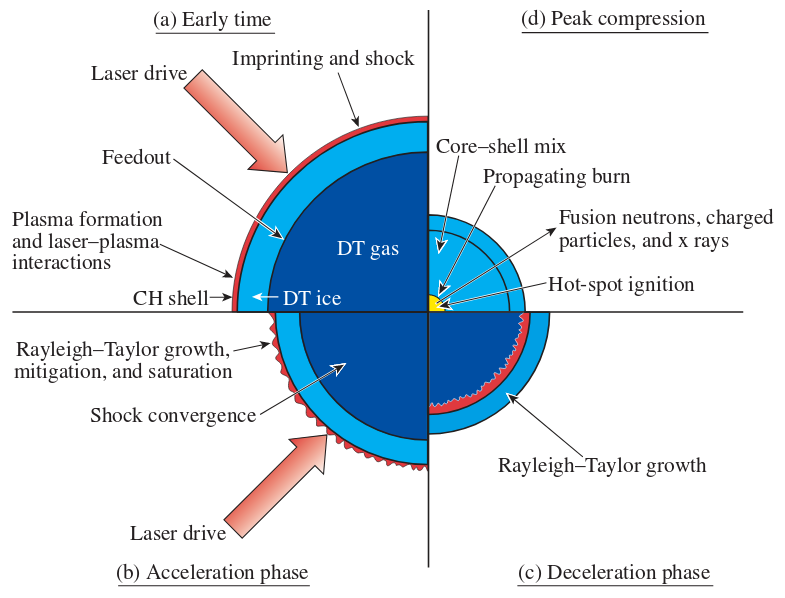
\includegraphics[width=0.55\linewidth]{../fig/DDfusion}
   \centering
  \end{figure}
 \footnote{\cite{craxton2015}}


\end{frame}


\section{Previous Equation System \& Modeling Capabilities}

\begin{frame}[t]{Eqn System $-$ 1 PreExisting FVM code}
  \minipage{\textwidth}
  \minipage{0.42\textwidth}
  \begin{align*}
    \pfrac{\rho}{t} + \nabla \cdot \left[\rho \mathbf{u}\right] &= 0 \\
    \pfrac{\rho \mathbf{u}}{t} + \nabla \cdot \left[\rho \mathbf{u}\mathbf{u}^T + \mathbb{I}P\right] = 0 \\
    \pfrac{\epsilon}{t} + \nabla \cdot \left[\left(\epsilon + P \right)\mathbf{u}\right] &= 0 \\
    \epsilon = \epsilon_{internal} + \frac{1}{2}\rho|\mathbf{u}|^2 &\\
    P = \rho \epsilon_{internal} (\gamma - 1) &
  \end{align*}
  \endminipage\hfill
  \minipage{0.57\textwidth}
 \begin{figure}[!htbp]
   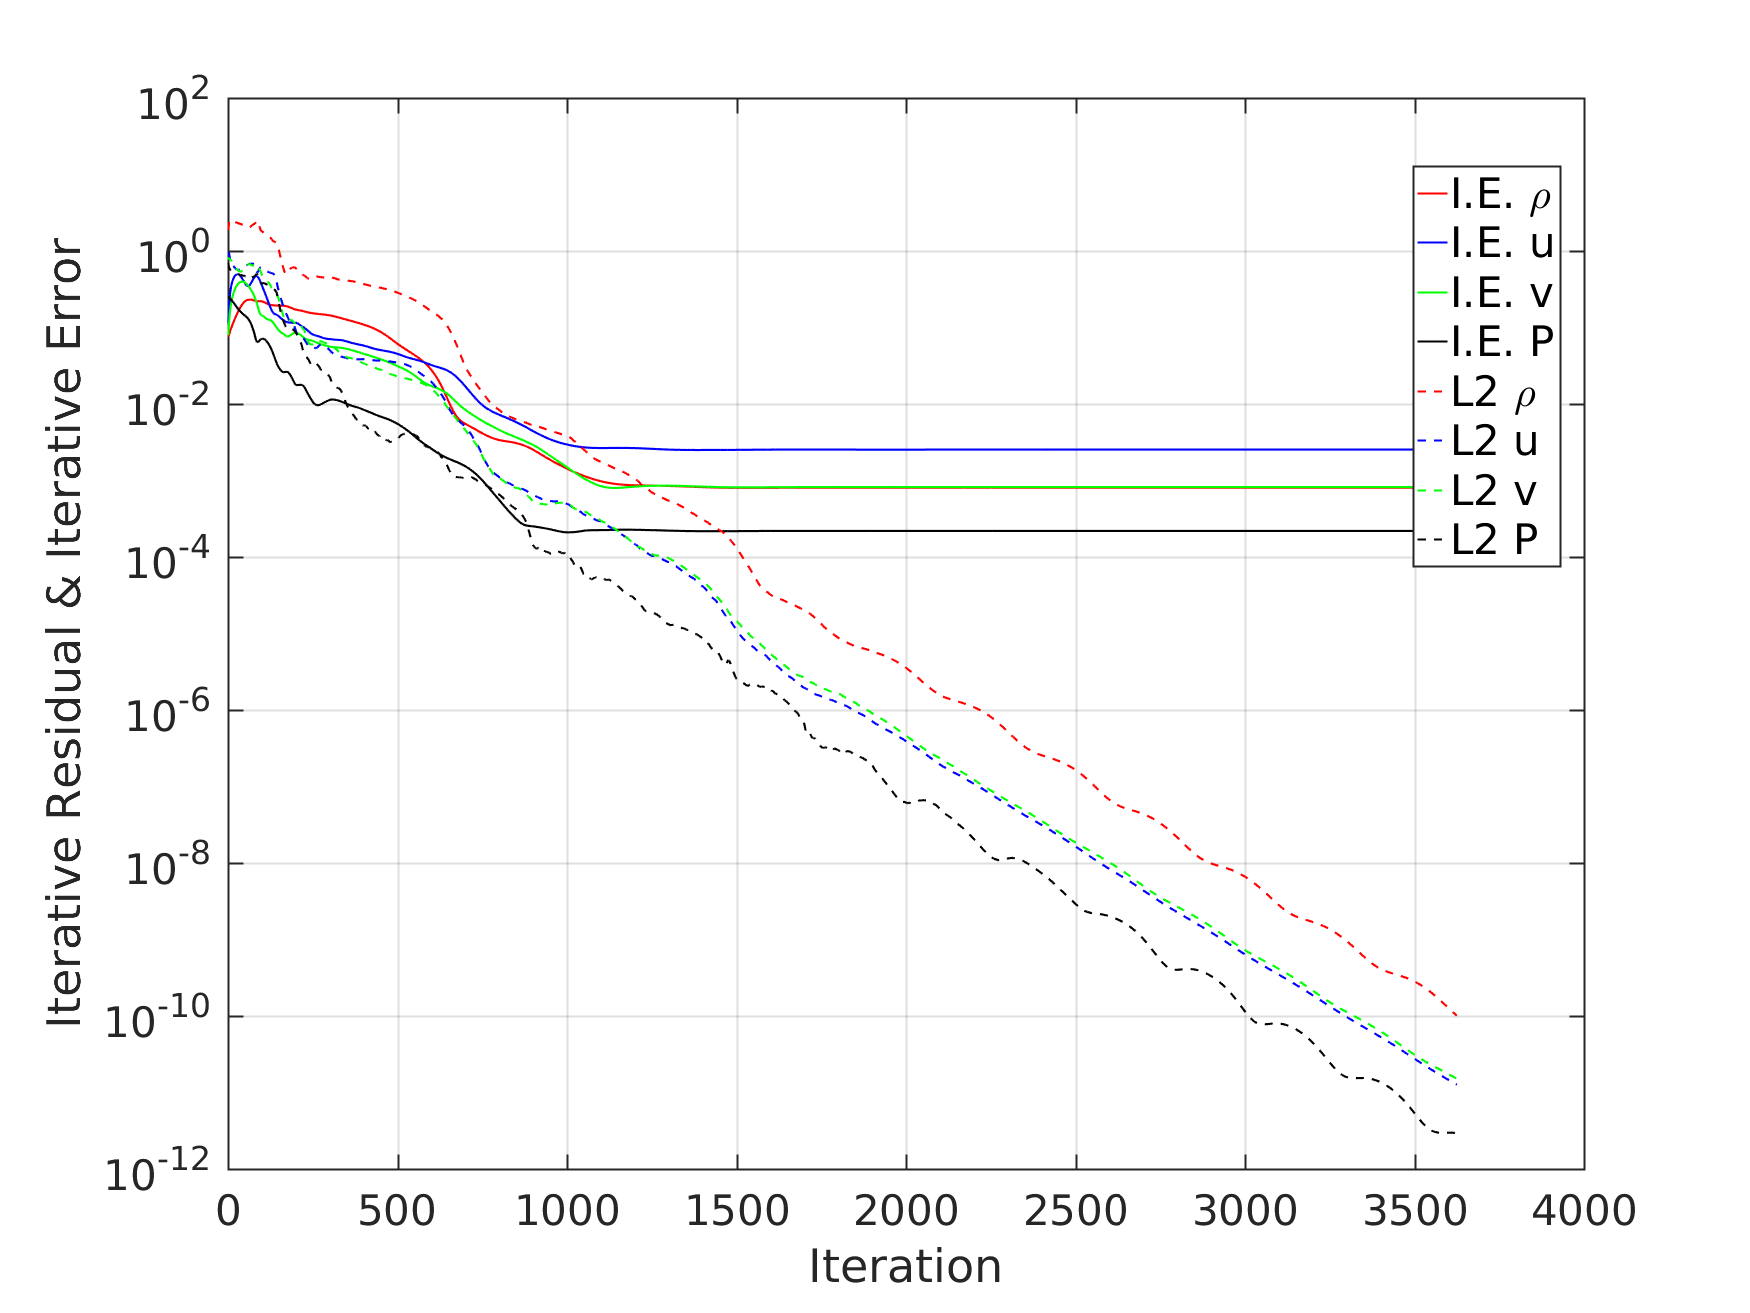
\includegraphics[width=1.0\linewidth]{fig/Iter_SB}
   \centering
 \end{figure}

  \endminipage\hfill
  \endminipage

\end{frame}

\begin{frame}[t]{Eqn System $-$ 2 PreExisting FVM code}
  \minipage{\textwidth}
  \minipage{0.48\textwidth}
  \begin{figure}[!htbp]
    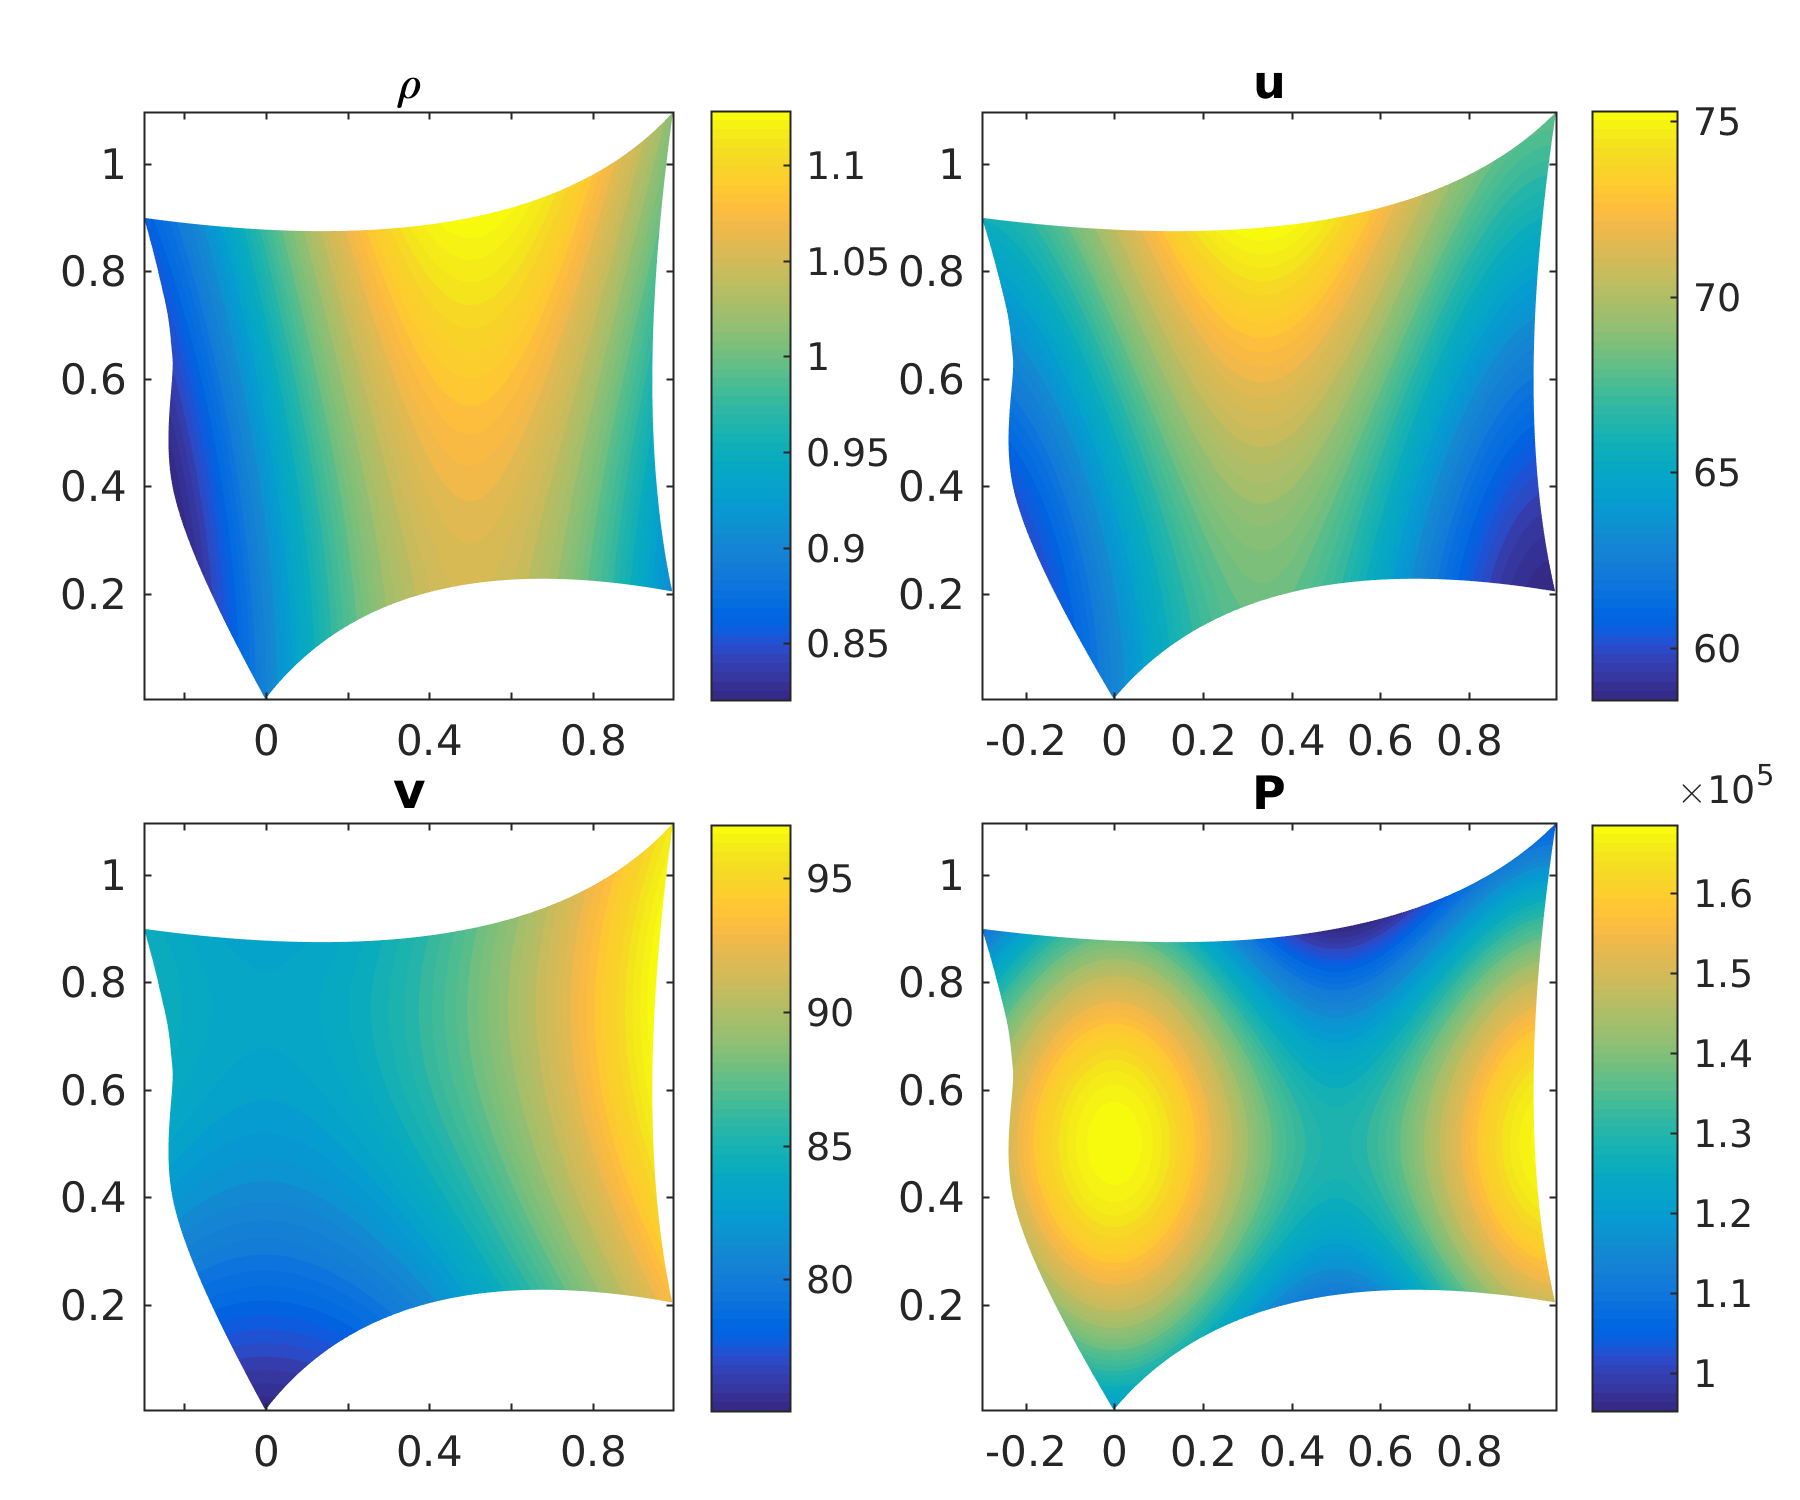
\includegraphics[width=1.0\linewidth]{fig/MMS_mesh6_SB_soln}
    \centering
  \end{figure}
  \endminipage\hfill
  \minipage{0.48\textwidth}
  \begin{figure}[!htbp]
    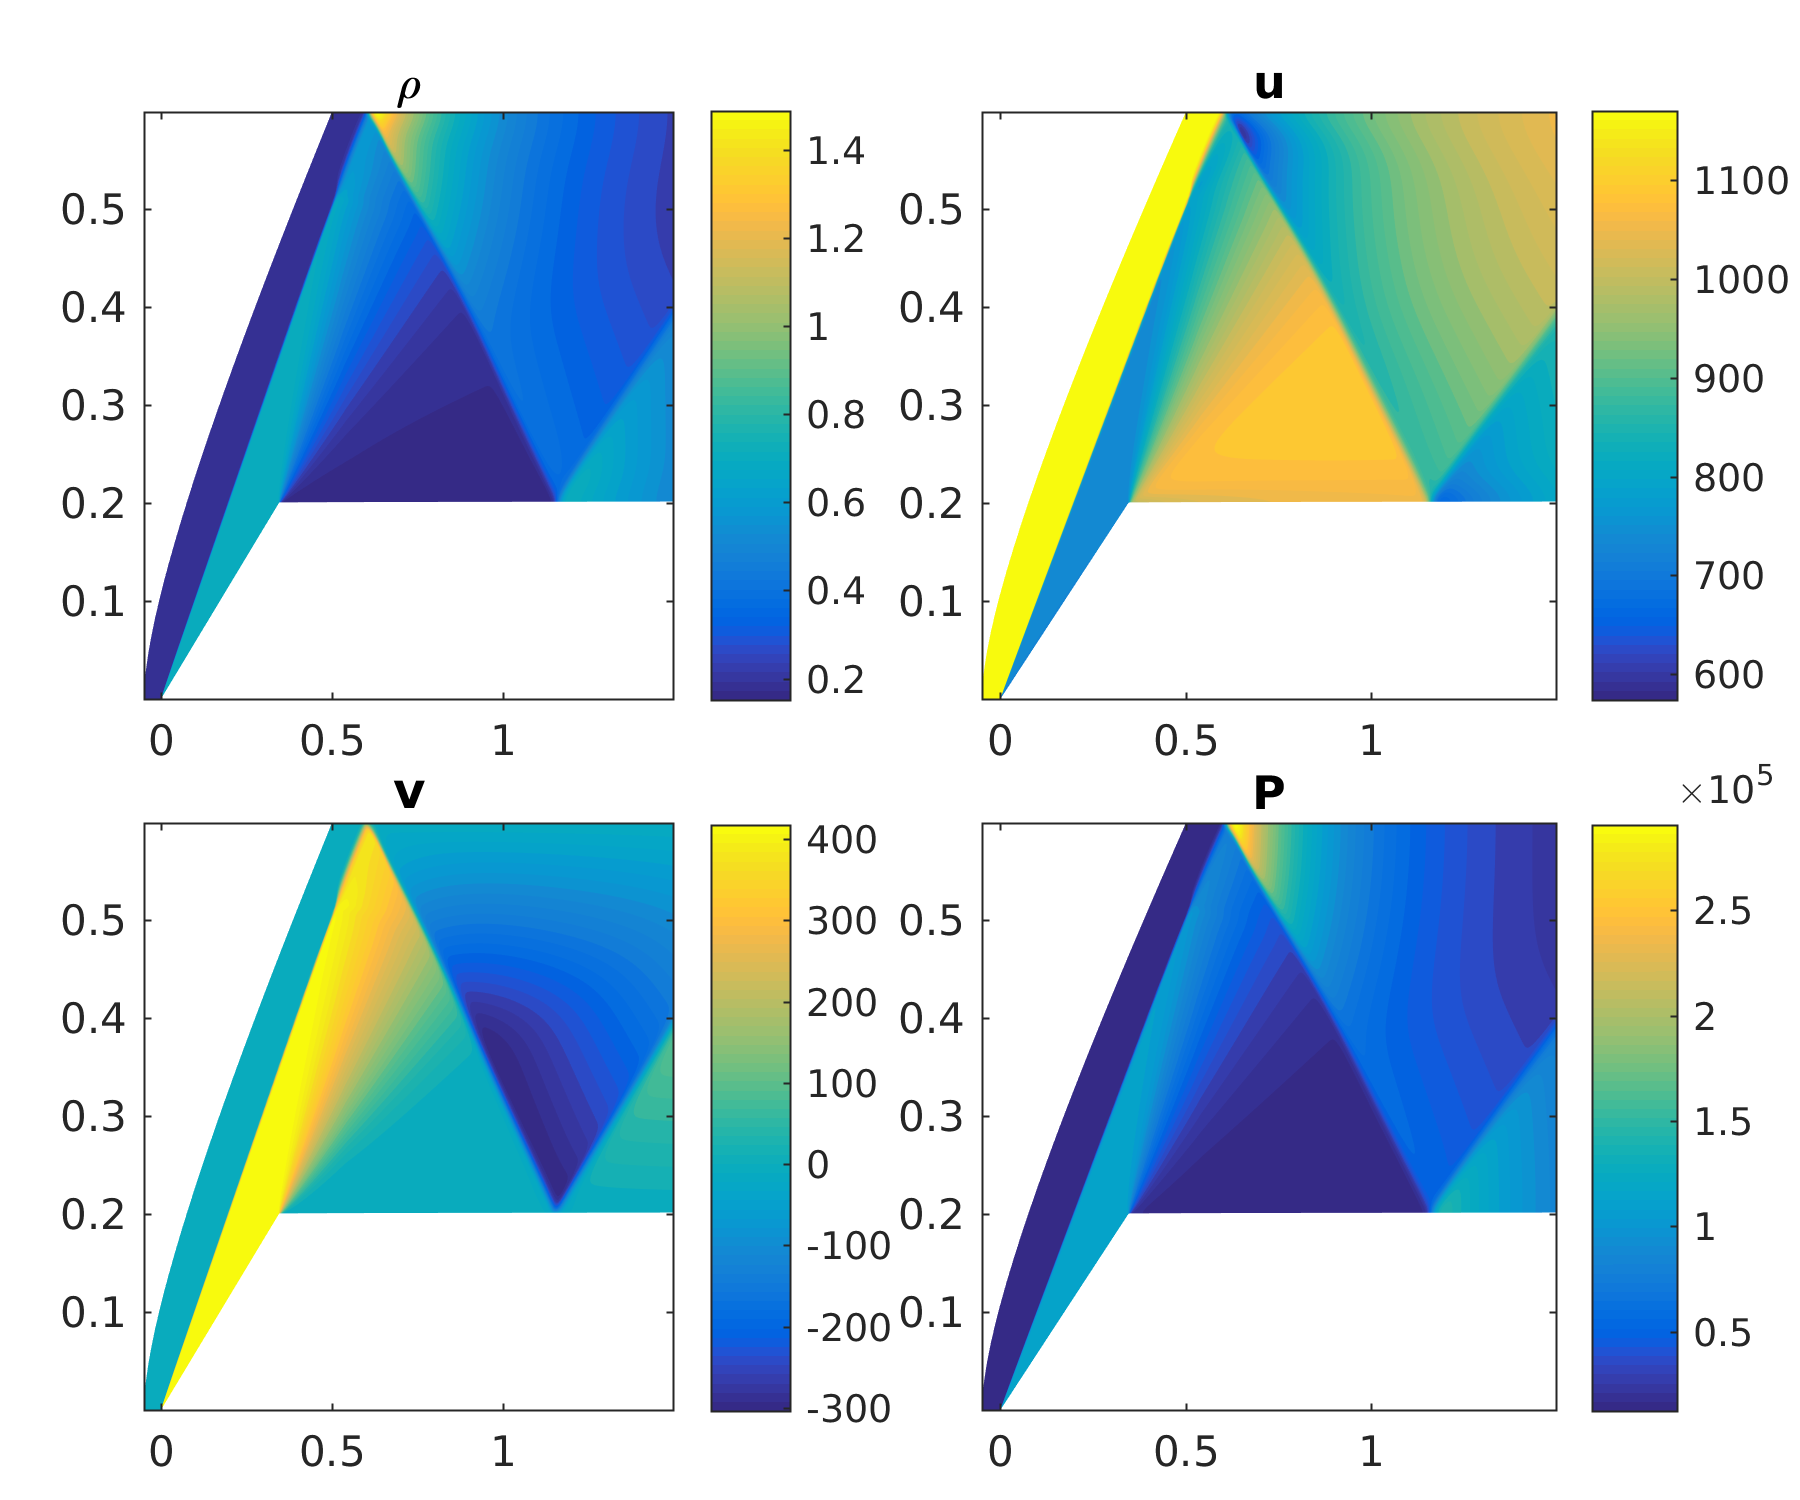
\includegraphics[width=1.0\linewidth]{fig/Inlet_mesh4_Soln}
    \centering
  \end{figure}
  \endminipage\hfill
  \endminipage
\end{frame}


\section{New Equation System \& Modeling Capabilities}

\begin{frame}[t]{Discretization $-$ 1}
 
 \vspace{-0.55cm}
  \begin{figure}[!htbp]
   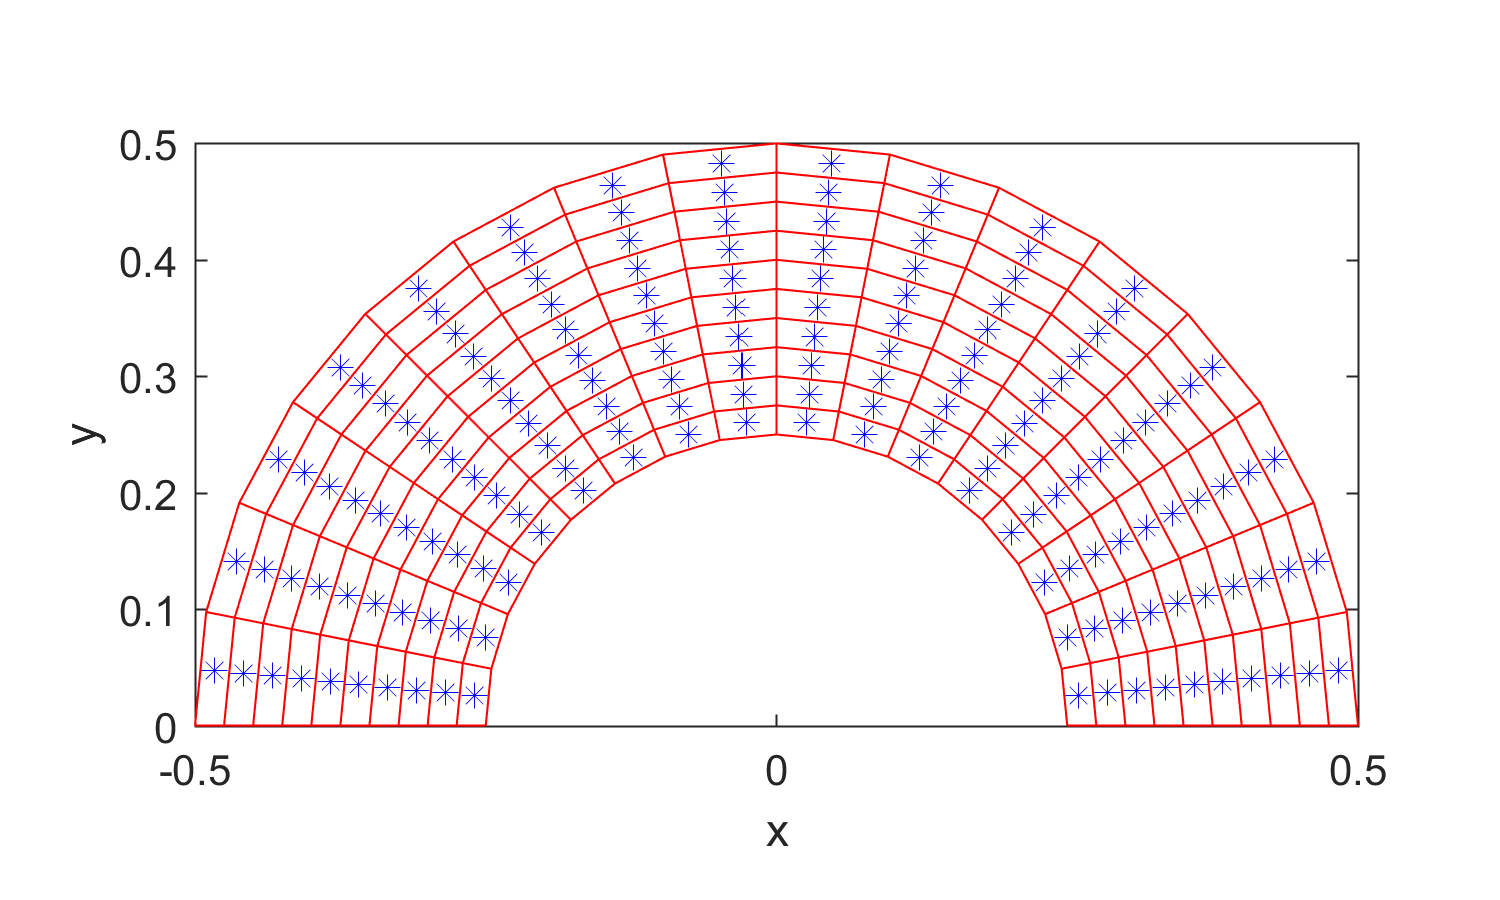
\includegraphics[width=0.85\linewidth]{../fig/16x10mesh}
   \centering
 \end{figure}

 \vspace{-0.5cm}
  \begin{itemize}
    \item Domain is discretized into cells which have constant averaged values
    \item Solves the integral form of the governing equations
  \end{itemize}

\end{frame}


\begin{frame}[t]{Discretization $-$ 2}
  \minipage{\textwidth}
    \minipage{0.48\textwidth}
    \textbf{Euler Equations $\rightarrow$ MHD}
      \begin{align*}
        \pfrac{\rho}{t} + \nabla \cdot \left[\rho \mathbf{u}\right] &= 0 \\
        \pfrac{\rho \mathbf{u}}{t} + \nabla \cdot \left[\rho \mathbf{u}\mathbf{u}^T + \mathbb{I}P\right] = 0 \\
        \pfrac{\epsilon}{t} + \nabla \cdot \left[\left(\epsilon + P \right)\mathbf{u}\right] &= 0 \\
        \epsilon = \epsilon_{internal} + \frac{1}{2}\rho|\mathbf{u}|^2 &\\
        P = \rho \epsilon_{internal} (\gamma - 1) &
      \end{align*}
    \endminipage\hfill
    \minipage{0.48\textwidth}
      \begin{align*}
        \pfrac{\rho}{t} + \nabla \cdot \left[\rho \mathbf{u}\right] &= 0 \\
        \pfrac{\rho \mathbf{u}}{t} + \nabla \cdot \left[\rho \mathbf{u}\mathbf{u}^T - \mathbf{b}\mathbf{b}^T + \mathbb{I}\left(P + \frac{1}{2}|\mathbf{b}|^2\right)\right] &= 0 \\
        \pfrac{\epsilon}{t} + \nabla \cdot \left[\left(\epsilon + P + \frac{1}{2}|\mathbf{b}|^2\right)\mathbf{u}- \mathbf{b}\cdot\mathbf{u}\mathbf{b}\right] &= 0 \\
        \pfrac{\mathbf{b}}{t} + \nabla\cdot\left[\mathbf{u}\mathbf{b}^T-\mathbf{b}\mathbf{u}^T\right] &= 0\\
        \epsilon = \epsilon_{internal} + \frac{1}{2}\rho|\mathbf{u}|^2 + \frac{1}{2}|\mathbf{b}|^2 
      \end{align*}
    \endminipage\hfill
  \endminipage
  \begin{equation*}
    \text{In short hand notation:}\;\pfrac{\mathbf{Q}}{t} + \nabla \cdot \rttensor{T} = 0, \; \mathbf{Q} = [\rho,\;\rho \mathbf{u},\; \epsilon,\;\mathbf{b}]^T, \; \&\; \rttensor{T} = [\cdots]^T
  \end{equation*}
\end{frame}

\begin{frame}[t]{Discretization $-$ 3}
  \textbf{2D Cartesian Flux Form}: $\pfrac{\mathbf{Q}}{t} + \pfrac{\mathbf{F}}{x} + \pfrac{\mathbf{G}}{y} = 0$ 
\[
  \pfrac{}{t}
  \begin{bmatrix}
    \rho  \\
    \rho u  \\
    \rho v \\
    \rho w \\
    \epsilon\\
    b_x \\
    b_y \\
    b_z 
  \end{bmatrix}
  \;+\;\pfrac{}{x}
  \begin{bmatrix}
    \rho u  \\
    \rho u^2 + P + \frac{1}{2}|\mathbf{b}|^2 - b_x^2\\
    \rho u v - b_x b_y \\
    \rho u w - b_x b_z \\
    \left(\epsilon+ P + \frac{1}{2}|\mathbf{b}|^2 \right) u - b_x \mathbf{u}\cdot\mathbf{b}\\
    0 \\
    b_y u - b_x v \\
    b_z u - b_x w 
  \end{bmatrix}
  \;+\;\pfrac{}{y}
  \begin{bmatrix}
    \rho v  \\
    \rho v u - b_y b_x\\
    \rho v^2 + P + \frac{1}{2}|\mathbf{b}|^2 - b_y^2\\
    \rho v w - b_y b_z \\
    \left(\epsilon+ P + \frac{1}{2}|\mathbf{b}|^2  \right) v - b_y\mathbf{u}\cdot\mathbf{b}\\
    b_x v - b_y u \\
    0 \\
    b_z v - b_y w 
  \end{bmatrix}
  =0
\]
mapping with curvilinear coordinates is covered in the report, but the integral form is given by
\begin{equation*}
  \oiiint \pfrac{\mathbf{Q}}{t} dV + \oiint \mathbf F dA_{\hat{x}}  + \oiint \mathbf G dA_{\hat{y}}  = 0
\end{equation*}
\end{frame}

\begin{frame}[t]{Discretization $-$ 4}
  \minipage{\textwidth}
  \minipage{0.35\textwidth}
  \textbf{Notes on FVM Scheme}
  \begin{itemize}
    \item Time Integration - 4 stage RK scheme
    \item Interface Reconstruction - Monotonic Upwind Scheme for Conservation Laws (MUSCL) 2nd order accurate (5 point stencil)
    \item Flux Form - Harten-Lax-Van leer (HLL) Approximate Riemann Solver ( 3 wave )
  \end{itemize}


  \endminipage\hfill
  \minipage{0.62\textwidth}
 \begin{figure}[!htbp]
   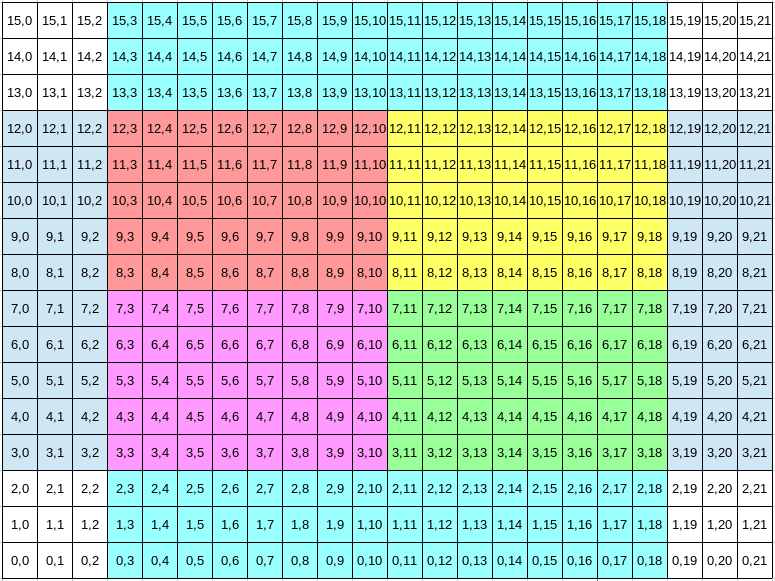
\includegraphics[width=1.0\linewidth]{../fig/16x10compDomain}
   \centering
 \end{figure}
  \endminipage\hfill
  \endminipage

\end{frame}


\section{Serial \& Parrallel}

\begin{frame}[t]{Serial $-$ 1}
  \textbf{Density growth at n = 1000}: Note - waves internal in heavy medium from perturbation
 \begin{figure}[!htbp]
   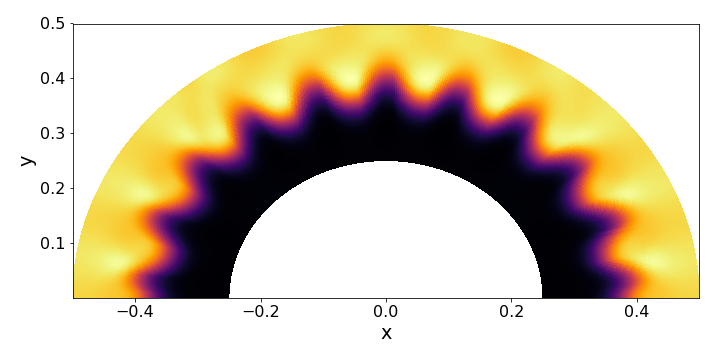
\includegraphics[width=0.85\linewidth]{fig/360x300serial}
   \centering
 \end{figure}

\end{frame}

\begin{frame}[t]{Parrallel $-$ 1}
  \vspace{-0.5cm}
 \begin{figure}[!htbp]
   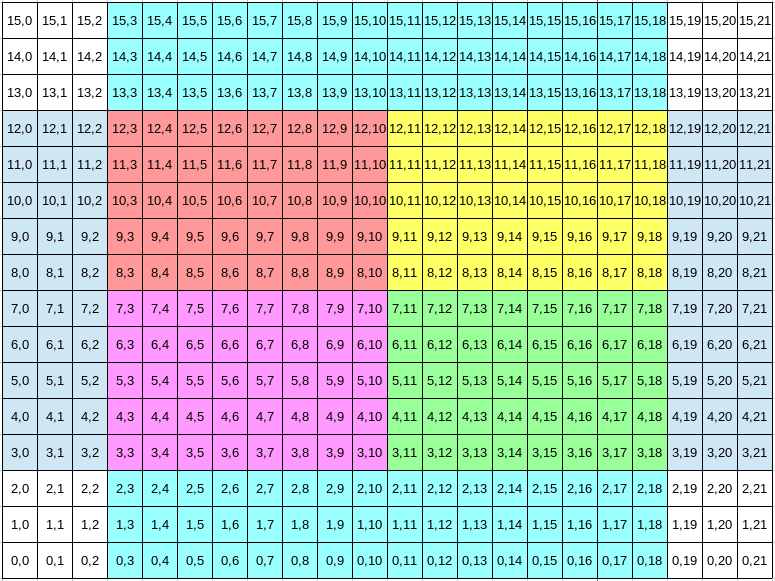
\includegraphics[width=0.65\linewidth]{../fig/16x10compDomain}
   \centering
 \end{figure}
\end{frame}

\begin{frame}[t]{Parrallel $-$ 2}
  \textbf{Density growth at n = 1000}: Note - Bug in H.E., I.O., and/or B.C.
 \begin{figure}[!htbp]
   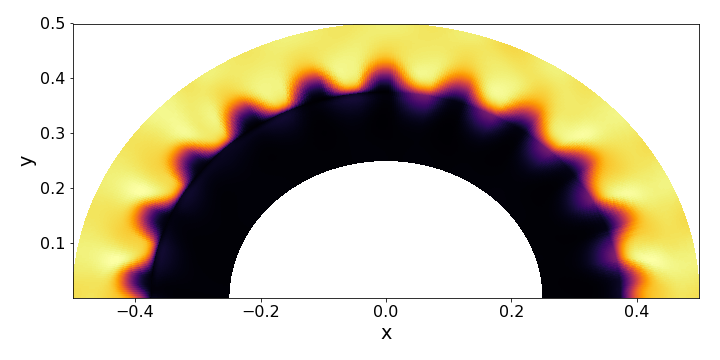
\includegraphics[width=0.85\linewidth]{fig/360x300parr}
   \centering
 \end{figure}
\end{frame}

\backupbegin

\begin{frame}[t,fragile]{References}

  \tiny
  \bibliographystyle{plainnat}
  \bibliography{../reference}
\end{frame}



\backupend






